\section{Model definition}
\label{model-definition}
This Section presents how the networks used on the dataset are 
structured and how the Hyperparameter tuning were performed.

\subsection{Neural network structure}
The starting point for the neural network structure was a 
reasonable network in terms of hidden layers. 
The rule of thumb followed to decide hidden neurons quantity is the 
following: 
$$\#\mathit{hidden\; neurons} = \frac{2}{3}\#\mathit{input\;neurons}
+ \#\mathit{output\;neurons}$$
The next step was to decide the hidden layer number. To respect the number of hidden 
neurons, 2 hidden layers were considered. More layers would mean 
having a real small number of neurons per layer, so 2 were preferred.

To give reference, this is the model used on the PCA training set, with 
120 input features.

\begin{center}
    
    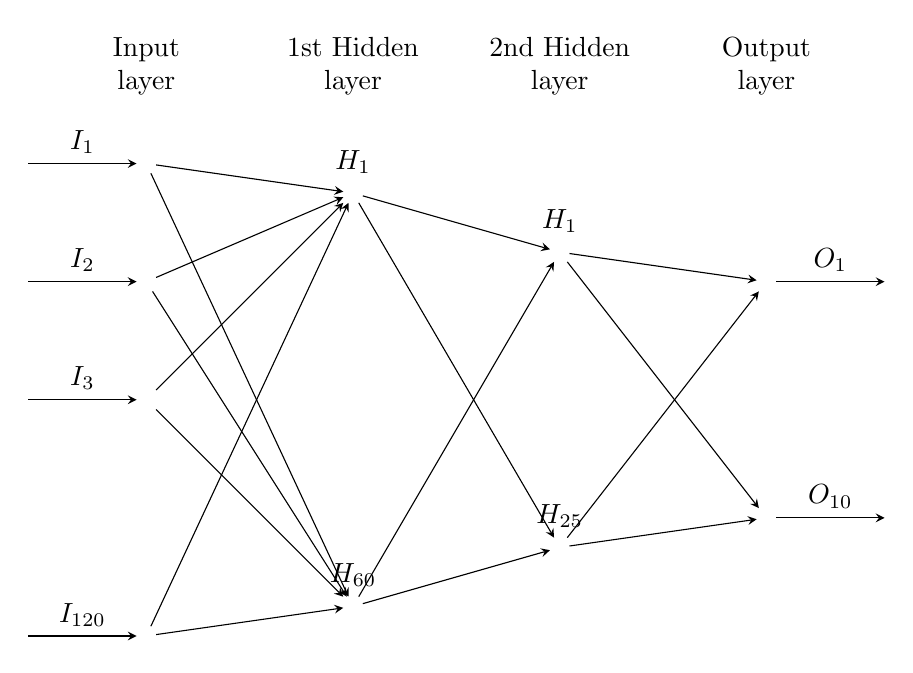
\begin{tikzpicture}[x=1.5cm, y=1.5cm, >=stealth]
        
        % layers
        \foreach \m/\l [count=\y] in {1,2,3,missing,4}
        \node [every neuron/.try, neuron \m/.try] (input-\m) at (0,2.5-\y) {};
        
        \foreach \m [count=\y] in {1,missing,2}
        \node [every neuron/.try, neuron \m/.try ] (hidden-\m) at (1.75,3-\y*1.75) {};
        
        \foreach \m [count=\y] in {1,missing,2}
        \node [every neuron/.try, neuron \m/.try ] (hidden2-\m) at (3.5,2-\y*1.25) {};
        
        \foreach \m [count=\y] in {1,missing,2}
        \node [every neuron/.try, neuron \m/.try ] (output-\m) at (5.25,1.5-\y) {};
        
        %   label
        \foreach \l [count=\i] in {1,2,3,{120}}
        \draw [<-] (input-\i) -- ++(-1,0)
        node [above, midway] {$I_{\l}$};
        
        \foreach \l [count=\i] in {1,60}
        \node [above] at (hidden-\i.north) {$H_{\l}$};
        
        \foreach \l [count=\i] in {1,25}
        \node [above] at (hidden2-\i.north) {$H_{\l}$};
        
        \foreach \l [count=\i] in {1,10}
        \draw [->] (output-\i) -- ++(1,0)
        node [above, midway] {$O_{\l}$};
        
        \foreach \i in {1,...,4}
        \foreach \j in {1,...,2}
        \draw [->] (input-\i) -- (hidden-\j);
        
        \foreach \i in {1,...,2}
        \foreach \j in {1,...,2}
        \draw [->] (hidden-\i) -- (hidden2-\j);
        
        \foreach \i in {1,...,2}
        \foreach \j in {1,...,2}
        \draw [->] (hidden2-\i) -- (output-\j);
        
        \foreach \l [count=\x from 0] in {Input, 1st Hidden, 2nd Hidden, Output}
        \node [align=center, above] at (\x*1.75,2) {\l \\ layer};
        
    \end{tikzpicture}
\end{center}
    

The activation function for the hidden layers is a \emph{Relu} and the last one 
is a \emph{softmax}. 
The loss used is the \emph{Sparse Categorical Crossentropy loss} as it is suited for this 
kind of problems.

As discussed in the previous Section, models with this logic for 
construction were tested on the four training sets to choose the one to tune 
the final network.

\subsection{Hyperparameter tuning}
\dots